\section{DVCS spin observables}\label{sec_dvcs_obs}
%\chead[\ref{sec_dvcs_obs} DVCS spin observables]{\let\uppercase\relax\leftmark}
A complete analysis of DVCS observables, including the asymmetries of interest in this document, in terms of Fourier harmonics with respect to the azimuthal angle, was carried out by Belitsky {\it et al.} \cite{belitski}, up to twist-3 approximation. 
These asymmetries allow the extraction of separate components of the azimuthal angular dependence of the $eN \to eN'\gamma$ cross section, which are related to the Compton Form Factors (CFFs) defined in Eqs.~\ref{def_cffs1}-\ref{def_cffs2}.% The cross section for exclusive photon production 
%\begin{eqnarray}
%\label{WQ}
%\frac{d\sigma}{d x_B dy dt d\phi}
%=
%\frac{\alpha^3  x_B y } {16 \, \pi^2 \,  Q^2 \sqrt{1 + \epsilon^2}}
%\left| \frac{\cal T}{e^3} \right|^2 \, 
%\end{eqnarray}
%depends on the Bjorken variable $x_B$, the squared momentum transfer $t =  (P_1 - P_2)^2$ (where $P_1$ and $P_2$ are the four-momenta of, respectively, the initial and final nucleon), the lepton energy fraction $y= P_1\cdot q_1/P_1\cdot k$, with $q_1 = k - k'$ (where $k$ and $k'$ are the four momenta of, respectively, the incoming and scattered electon) and the angle $\phi$, which is the angle between the leptonic and hadronic planes, as shown in Fig.~\ref{fig:dvcs_phi}. We define $\epsilon=2 x_B \frac{M}{Q}$. 
\begin{figure}[h]
\begin{center}
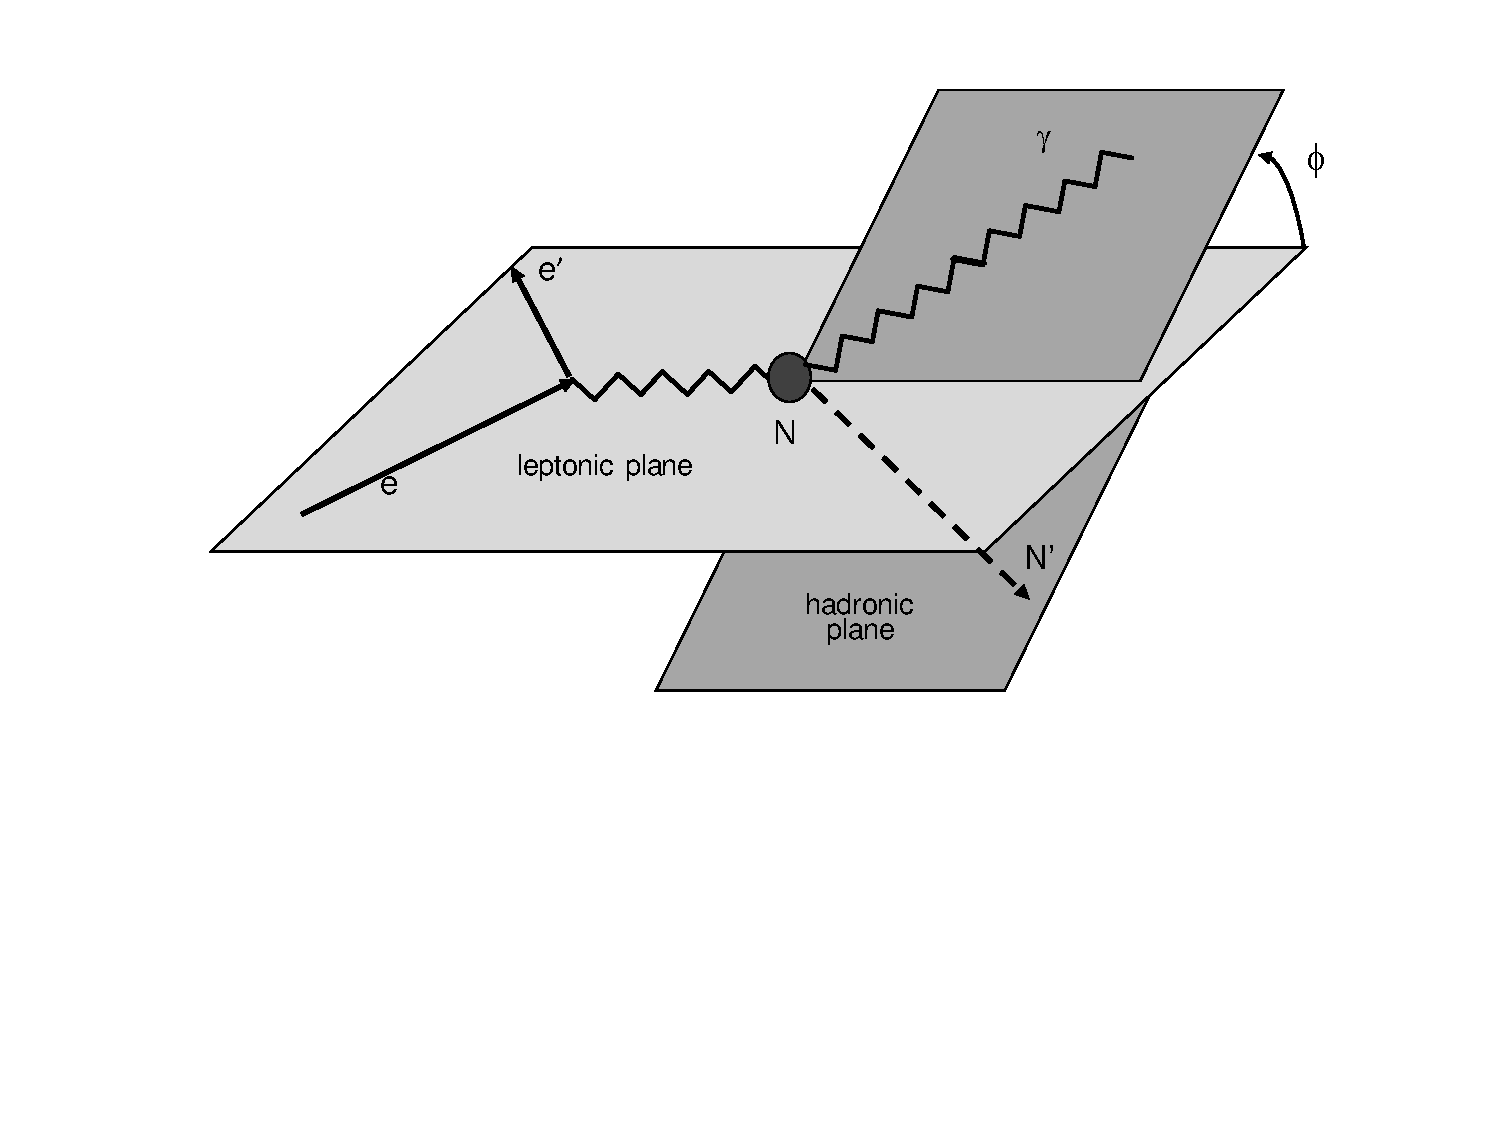
\includegraphics[width=120mm]{dvcs_diagram.pdf}
\vspace{-3.cm}
%\vskip -1cm
\caption[$eN \to eN'\gamma$ reaction plane.]{Schematic to illustrate the definition of the angle $\phi$, formed by the leptonic and hadronic planes, in the $eN \to eN'\gamma$ reaction.}
\label{fig:dvcs_phi}
\end{center}
\end{figure}

The amplitude ${\cal T}$ for the exclusive electroproduction of photons is the sum of the DVCS ${\cal T}_{\rm DVCS}$ and Bethe-Heitler (BH) ${\cal T}_{\rm BH}$ amplitudes:

%The azimuthal angular dependence of each of the three terms in
\begin{equation}
{\cal T}^2
= |{\cal T}_{\rm BH}|^2 + |{\cal T}_{\rm DVCS}|^2 + {\cal I}
\, ,
\end{equation}
where ${\cal I}$ is the interference term
\begin{equation}
{\cal I}
= {\cal T}_{\rm DVCS} {\cal T}_{\rm BH}^\ast
+ {\cal T}_{\rm DVCS}^\ast {\cal T}_{\rm BH}
\, .
\end{equation}
The azimuthal angular dependence of each of the three terms is given by \cite{belitski}:
\begin{eqnarray}
\label{Par-BH}
|{\cal T}_{\rm BH}|^2
&=& \frac{e^6}
{x_B^2 y^2 (1 + \epsilon^2)^2 t\, {\cal P}_1 (\phi) {\cal P}_2 (\phi)}
\{
c^{\rm BH}_0 + \nonumber \\
&+&  \sum_{n = 1}^2
c^{\rm BH}_n \, \cos{(n\phi)} + s^{\rm BH}_1 \, \sin(\phi)\},
\end{eqnarray}
\begin{eqnarray}
\label{AmplitudesSquared}
|{\cal T}_{\rm DVCS}|^2
&=& \frac{e^6}{y^2 {\cal Q}^2}\{c^{\rm DVCS}_0 + \sum_{n=1}^2 [c^{\rm DVCS}_n \cos (n\phi) + \nonumber\\
&+& s^{\rm DVCS}_n \sin (n \phi)]\} \, ,
\end{eqnarray}
\begin{eqnarray}
\label{InterferenceTerm}
{\cal I}&=& \frac{e^6}{x_B y^3 t {\cal P}_1 (\phi) {\cal P}_2 (\phi)}\{c_0^{\cal I}+ \sum_{n = 1}^3[c_n^{\cal I} \cos(n \phi) +\nonumber\\
&+&  s_n^{\cal I} \sin(n \phi)]\} \, ,
\end{eqnarray}
where $\phi$ is the angle between the leptonic and hadronic planes, as shown in Fig.~\ref{fig:dvcs_phi}, ${\cal P}_1$ and ${\cal P}_2$ are lepton BH propagators, $y= P_1\cdot q_1/P_1\cdot k$, where where $P_1$ is the four-momentum of the initial nucleon. For more details and definitions, see \cite{belitski}.
The Fourier coefficients in $|{\cal T}_{\rm BH}|^2$ are calculable in QED, with knowledge of the nucleon form factors, while the ones appearing in ${\cal I}$ and $|{\cal T}_{\rm DVCS}|^2$ depend on the Compton Form Factors. 

\subsection{Target-spin asymmetry}\label{sec_tsa}
The use of a longitudinally polarized (LP) target allows the extraction of the target-spin asymmetry $A_{UL}$ (here also referred to as TSA) which is given, at twist-2 level, by:
\begin{equation}\label{eq_tsa}
A_{\rm UL}(\phi) \sim \frac{s_{1,{\rm LP}}^{\cal I}\sin\phi}{c_{0,{\rm unp}}^{\rm BH}+(c_{1,{\rm unp}}^{\rm BH}+c_{1,{\rm unp}}^{\cal I}+...)\cos\phi+...}\ 
\end{equation}
where the ellipses in the denominator represent smaller terms. The $\sin\phi$ coefficient $s_{1,{\rm LP}}$, originating from the DVCS/BH interference term, at leading-twist is proportional to a linear combination of the imaginary parts of the four CFFs, 
\begin{eqnarray}
s_{1,{\rm LP}} &\propto&  \Im{\rm m}[ F_1\widetilde{\cal H}+\xi(F_1+F_2)({\cal H}+\frac{x_B}{2}{\cal E})+\nonumber \\
&-& \xi(\frac{x_B}{2} F_1+ \frac{t}{4M^2}F_2)\widetilde{\cal E}] ,
\end{eqnarray}
\noindent
where $F_1$ and $F_2$ are, respectively, the Dirac and Pauli form factors. In the case of a proton target, the dominant contribution to $A_{\rm UL}$ comes from $\Im{\rm m} \widetilde{\cal {H}}_p$ and from $\Im{\rm m}{\cal {H}}_p$. {\bf In the neutron case, for which $\boldsymbol{F_2 >> F_1}$, this observable is mostly sensitive to $\boldsymbol{\Im{\rm m}{\cal {H}}_n}$}. 

\subsection{Double-spin asymmetry}\label{sec_dsa}

The use of a polarized electron beam along with a polarized target allows also the determination of the double spin asymmetry $A_{\rm LL}$. Unlike $A_{\rm UL}$, the Bethe-Heitler process alone can generate a non-zero value for this observable. At twist-2 level, it takes the form: 

\begin{equation}
A_{LL}(\phi) \sim \frac{c_{0,{\rm LP}}^{\rm BH}+c_{0,{\rm LP}}^{\cal I}
	 +(c_{1,{\rm LP}}^{\rm BH}+c_{1,{\rm LP}}^{\cal I})\cos\phi}
	{c_{0,{\rm unp}}^{\rm BH}+(c_{1,{\rm unp}}^{\rm BH}+c_{1,{\rm unp}}^{\cal I}+...)\cos\phi...}
\end{equation}
with
\begin{eqnarray}\label{eq_dsa}
c_{0,{\rm LP}}^{\cal I}, c_{1,{\rm LP}}^{\cal I}
&\propto& \Re{\rm e} [F_1 \widetilde { \cal H} + \xi (F_1 +  F_2)({\cal H}+\frac{x_B}{2}{\cal E})+\nonumber\\
&-& \xi(\frac{x_B}{2} F_1+\frac{t}{4M^2}F_2)\widetilde{\cal E} ],
\end{eqnarray}
\noindent

In this expression, the interference terms are expected to be smaller than the known BH terms \cite{belitski}. Moreover, both the constant and the $\cos\phi$-dependent terms contain contributions from both BH and the DVCS/BH interference. Nonetheless, it is expected that in some parts of the phase space $A_{\rm LL}$ has a measurable sensitivity to $\Re{\rm e} \widetilde{\cal H}_p$ (and, in a lesser way, $\Re{\rm e}{\cal H}_p$), for the proton, {\bf and to $\boldsymbol{\Re{\rm e}{\cal H}_n}$ for the neutron}.
